%----------------------------------------------------------------------------------------
%	PACKAGES AND THEMES
%----------------------------------------------------------------------------------------
\documentclass[aspectratio=169,xcolor=dvipsnames]{beamer}
\usetheme{SimplePlus}

\usepackage{hyperref}
\usepackage{graphicx} % Allows including images
\usepackage{booktabs} % Allows the use of \toprule, \midrule and \bottomrule in tables
\setbeamerfont{block title}{size=\Huge}

\setbeamerfont{block body}{size=\Huge}

%----------------------------------------------------------------------------------------
%	TITLE PAGE
%----------------------------------------------------------------------------------------

\title[short title]{Spurious Solar-Wind Effects on Acceleration Noise in LISA Pathfinder
} % The short title appears at the bottom of every slide, the full title is only on the title page

\author{Indie Desiderio-Sloane and Arnold Yang}

\institute[NTU] % Your institution as it will appear on the bottom of every slide, may be shorthand to save space
{
   Institute for Computing in Research
}
\date{\today} % Date, can be changed to a custom date


%----------------------------------------------------------------------------------------
%	PRESENTATION SLIDES
%----------------------------------------------------------------------------------------

\begin{document}

\begin{frame}
    % Print the title page as the first slide
    \titlepage
\end{frame}
%------------------------------------------------
\begin{frame}{Newton}
    \centering
    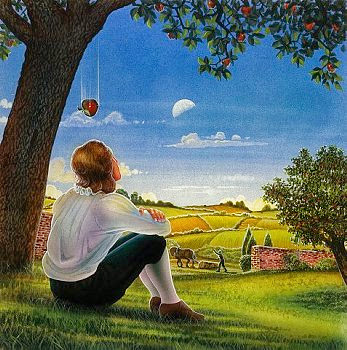
\includegraphics[height=7cm]{newton.jpg}
\end{frame}
%------------------------------------------------
\begin{frame}{Einstein}
    %\centering
    \begin{columns}[t]
    \begin{column}{3cm}

    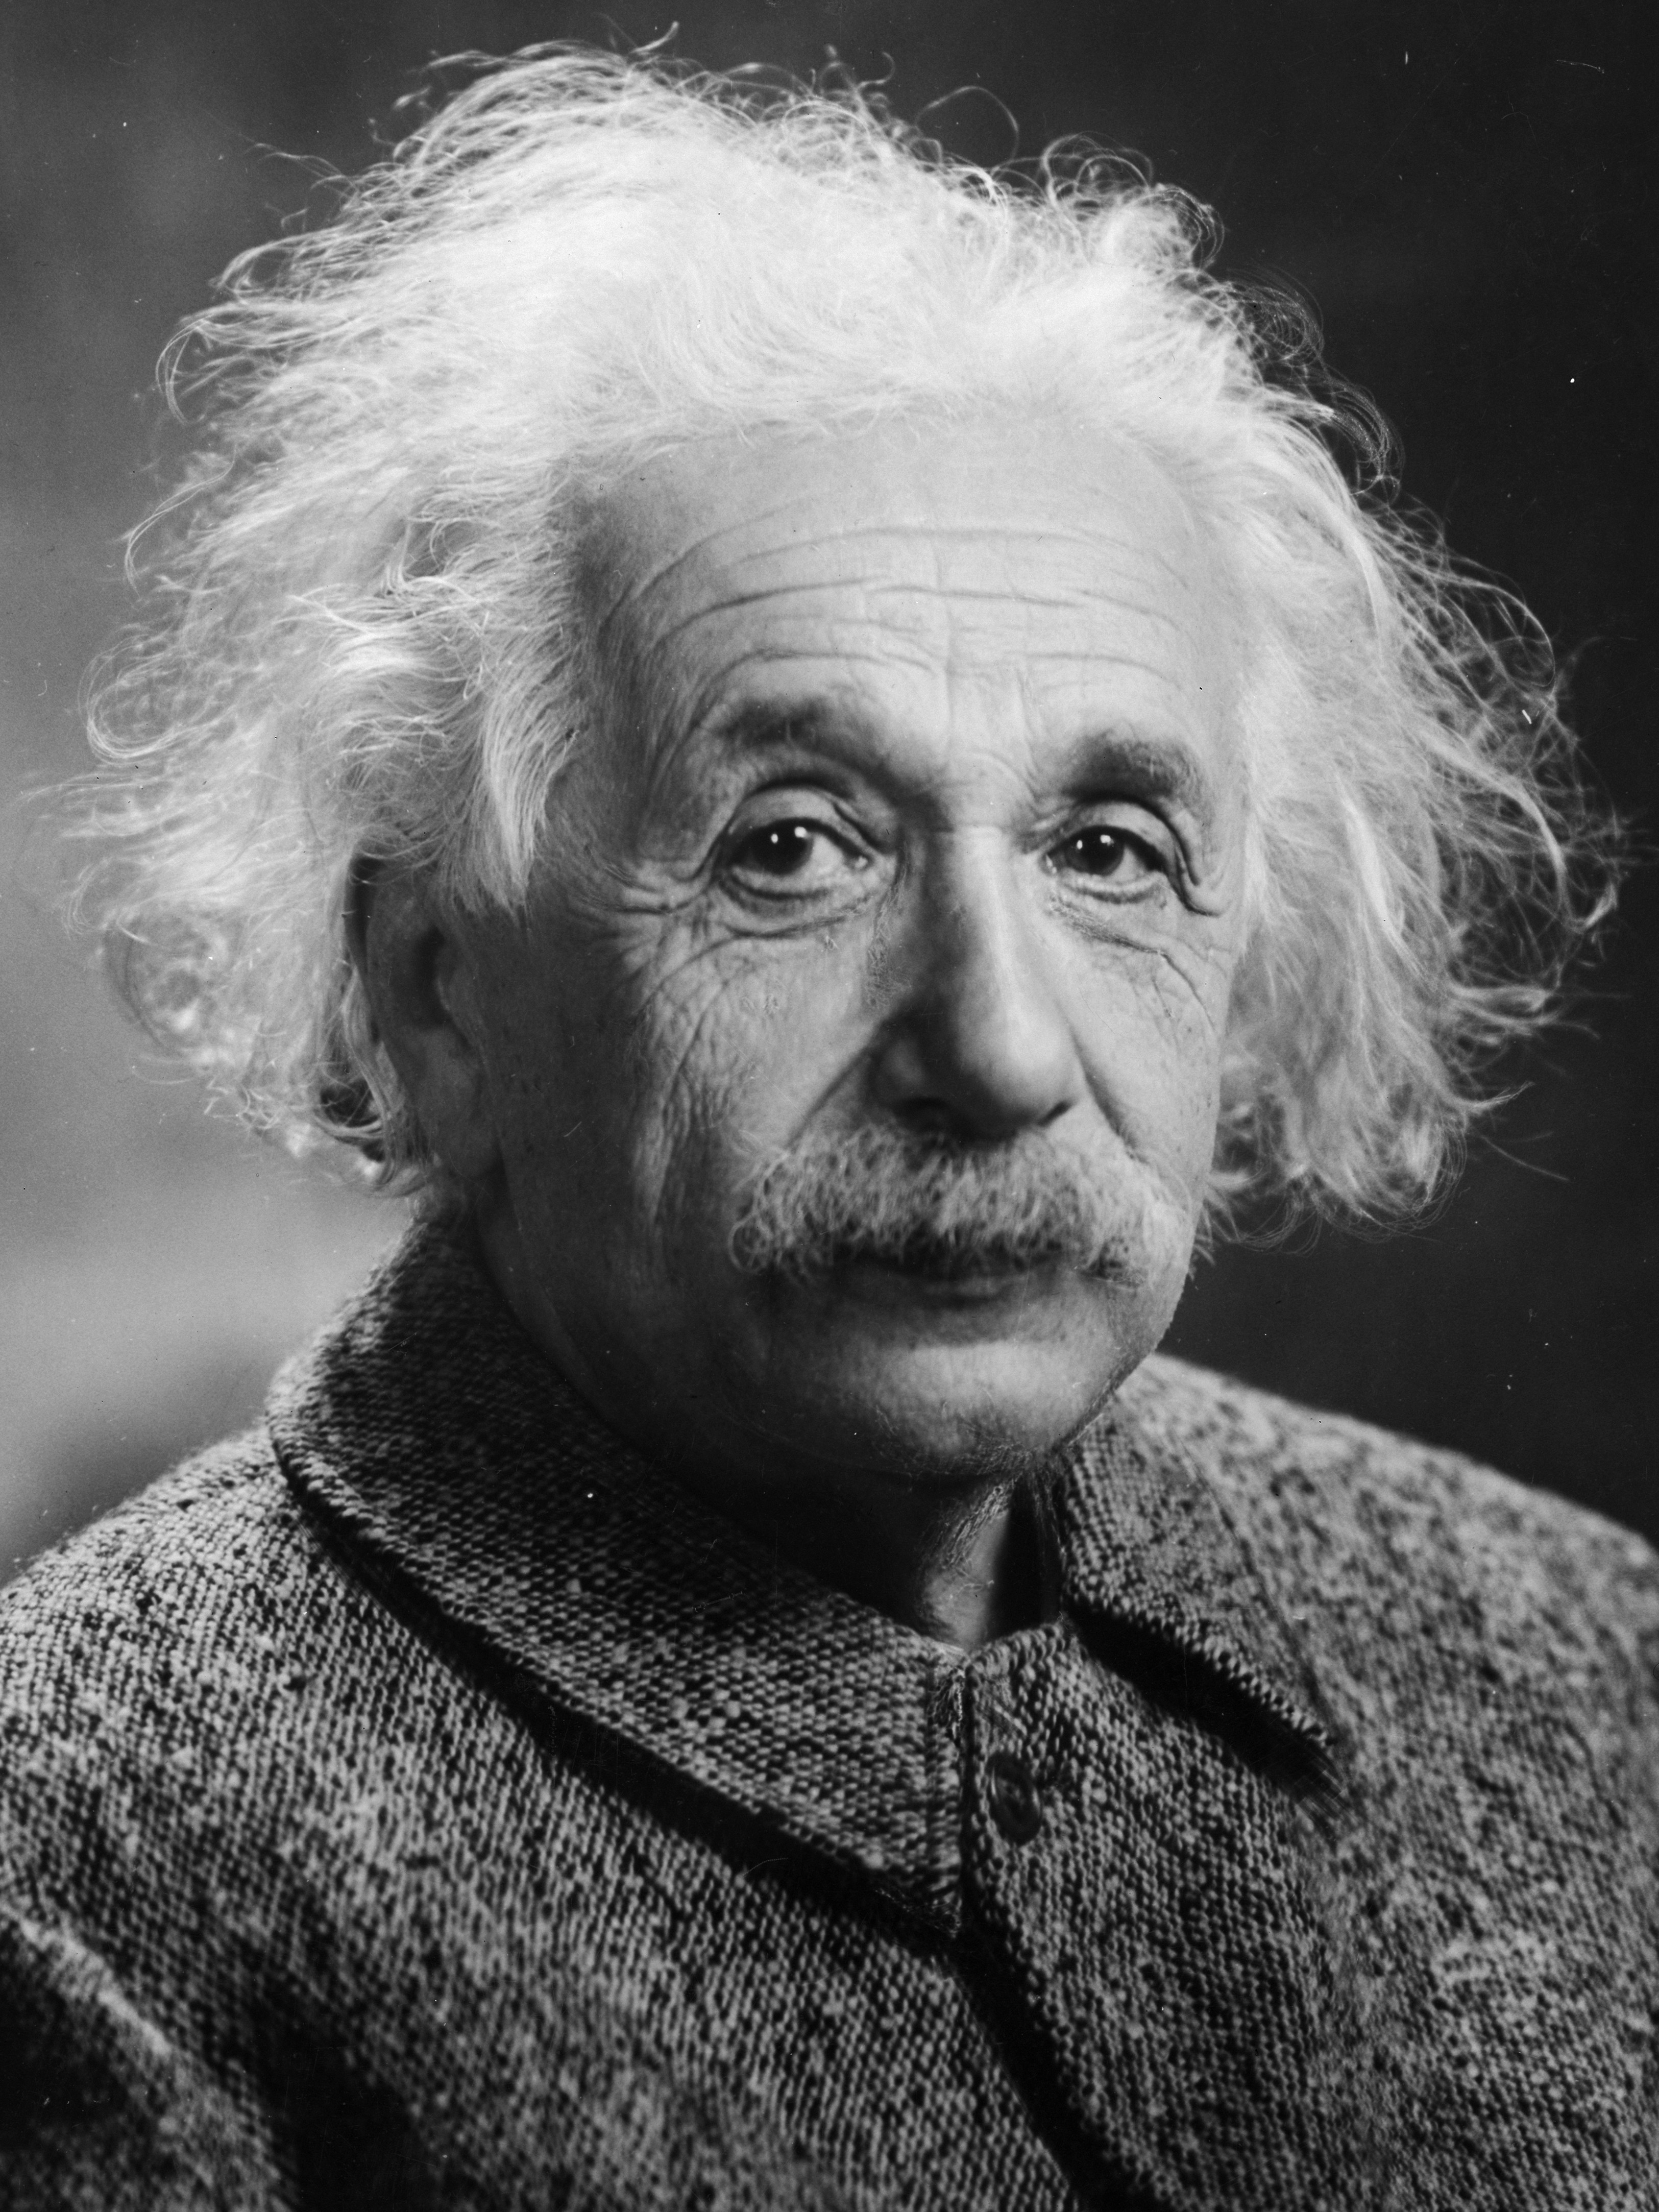
\includegraphics[height=6cm]{einstein.jpg}

    \end{column}
    \begin{column}{5cm}
    \begin{varblock}
    \Huge\[G_{\mu\nu}=\frac{8\pi G}{c{^4}}T_{\mu\nu}\]
    \end{varblock}

    \begin{varblock}
    \Huge\[h=\frac{2G}{c{^4}}\frac{1}{r}\frac{\delta{^2}Q}{\delta t{^2}}\]
    \end{varblock}
    \end{column}
    \end{columns}


\end{frame}

%------------------------------------------------
\begin{frame}{Cosmic Microwave Background}
   \centering
    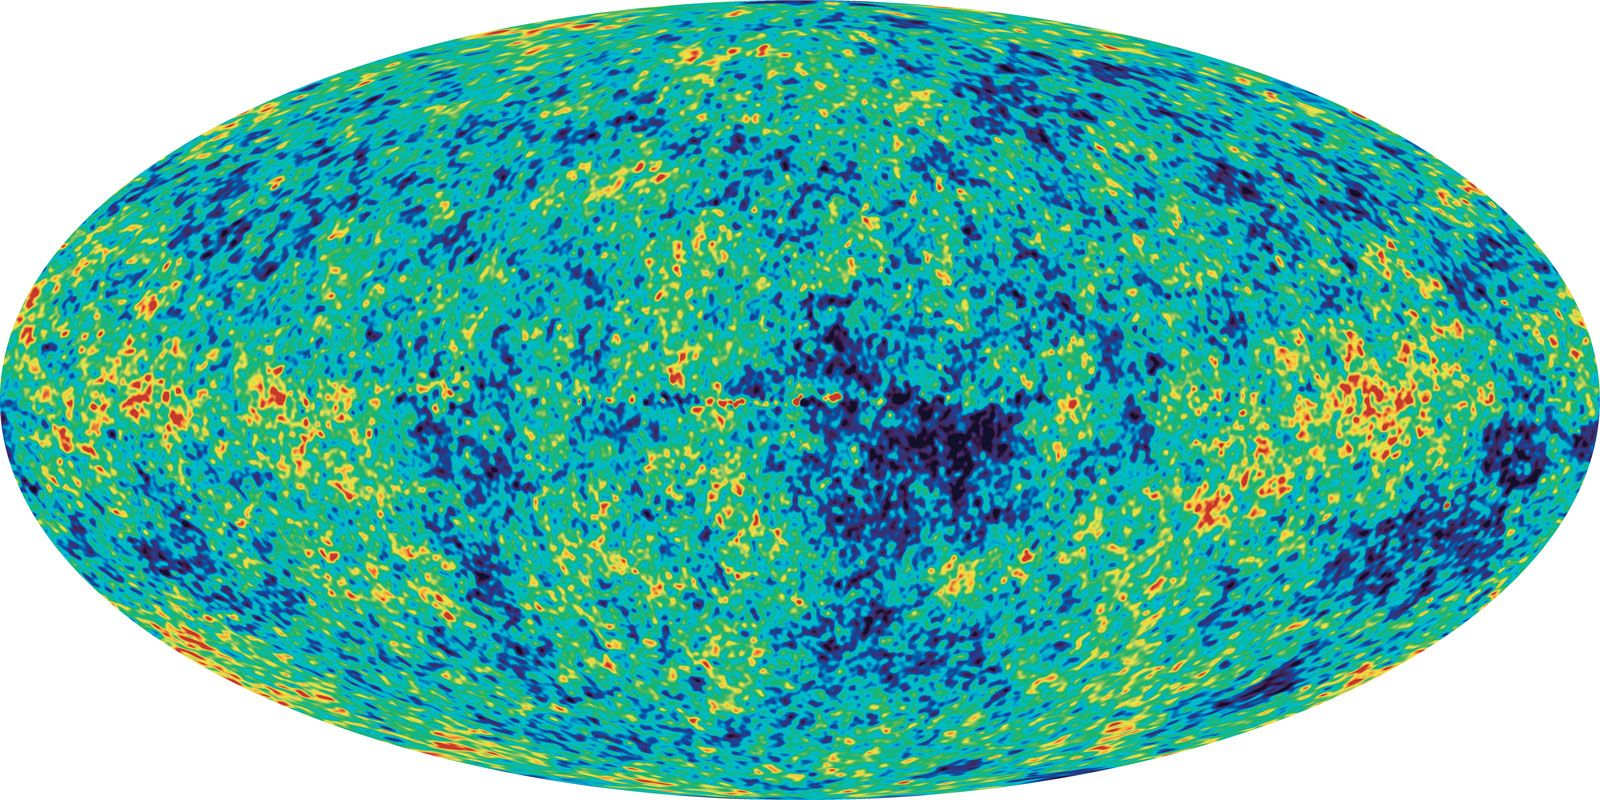
\includegraphics[height=7cm]{world.jpg}
\end{frame}
%------------------------------------------------
%------------------------------------------------
\begin{frame}{Cosmic Microwave Background}
   \centering
    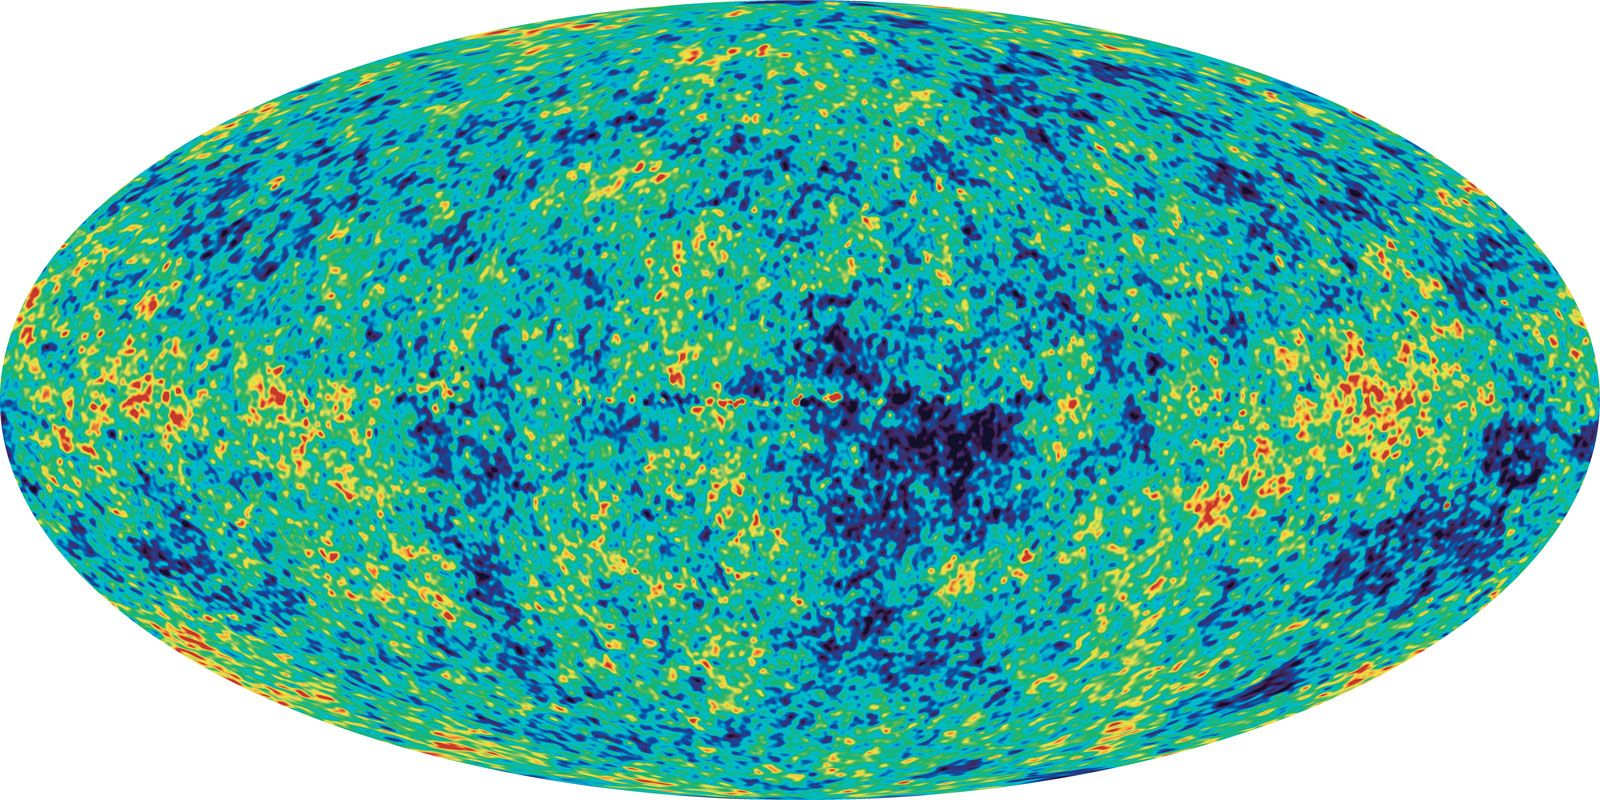
\includegraphics[height=7cm]{world.jpg}
\end{frame}
%------------------------------------------------
\begin{frame}{LIGO}
    \centering
    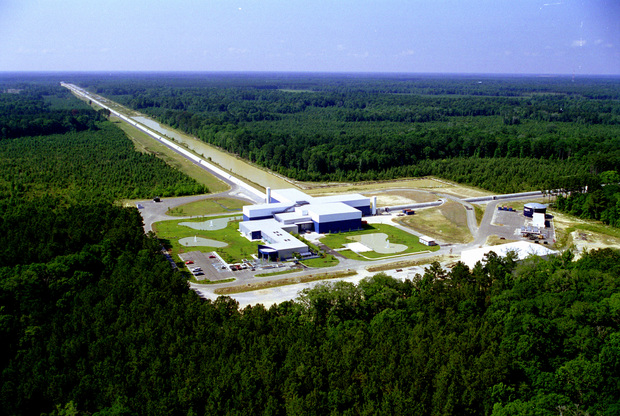
\includegraphics[height=7cm]{ligo.jpg}
\end{frame}
%------------------------------------------------
\begin{frame}{LISA}
    \centering
    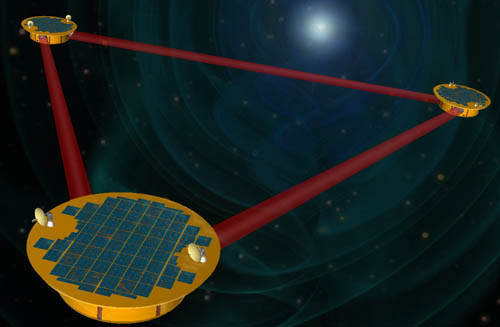
\includegraphics[height=7cm]{LISA.jpg}
\end{frame}
%------------------------------------------------
\begin{frame}{LISA Pathfinder}
    \centering
    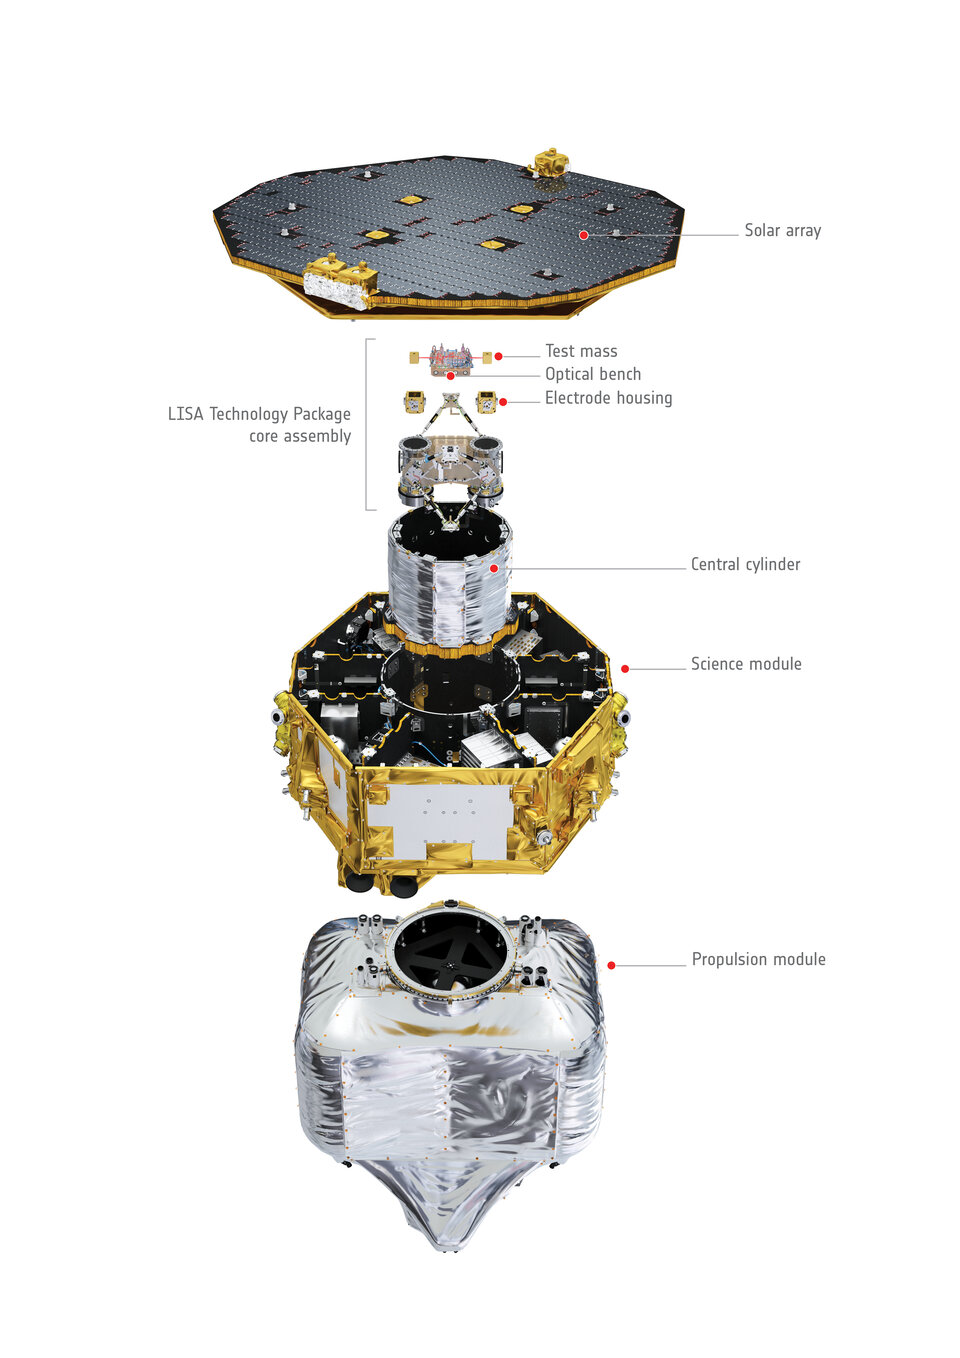
\includegraphics[height=7cm]{LPF.jpg}
\end{frame}
%------------------------------------------------
\begin{frame}{Solar Wind}
    \centering
    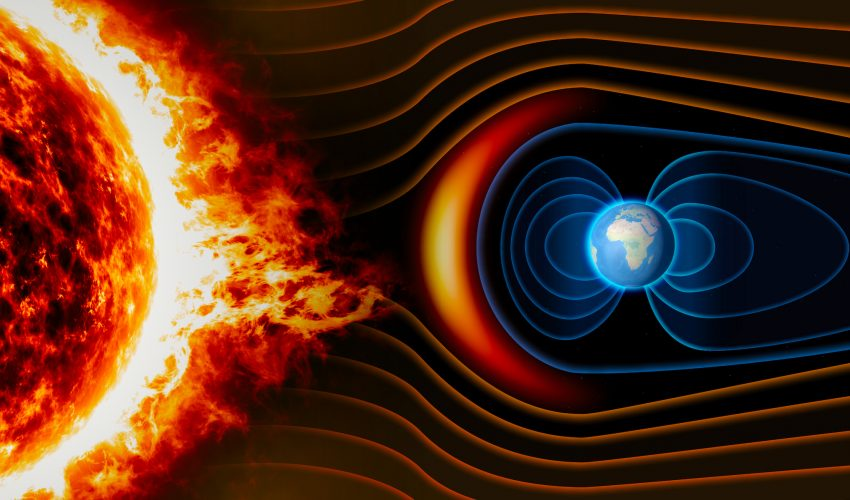
\includegraphics[height=7cm]{solarwind.jpg}
\end{frame}
%------------------------------------------------
\begin{frame}{ACE}
\centering
    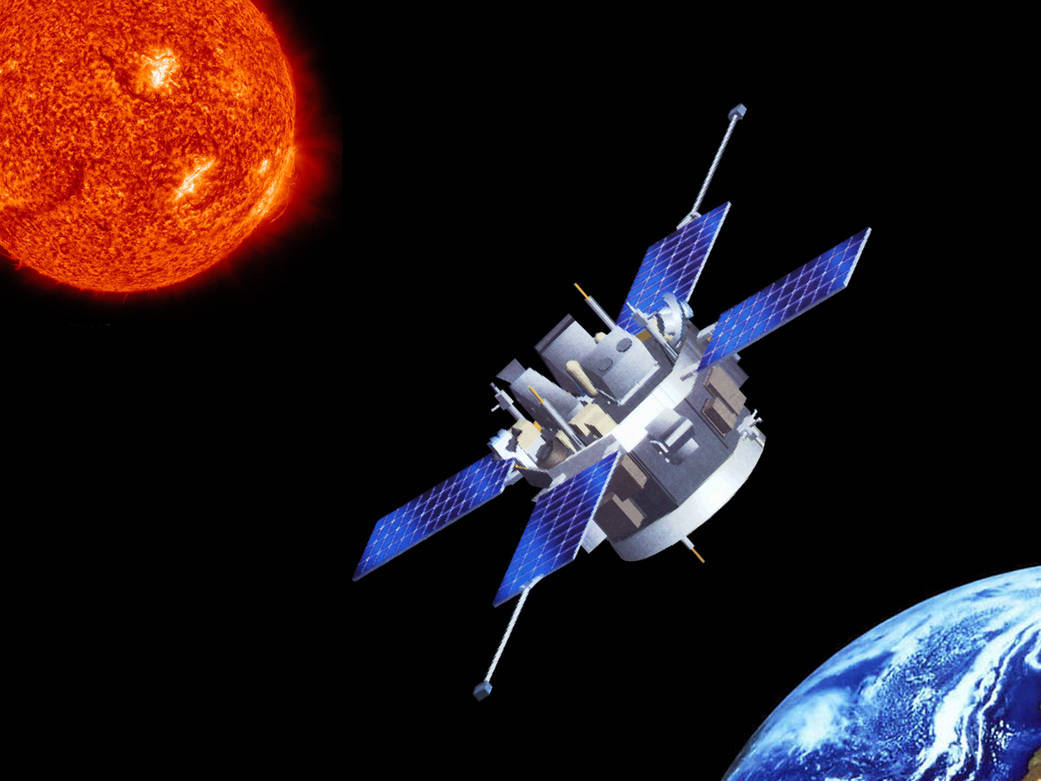
\includegraphics[height=7cm]{ACE.jpg}
\end{frame}
%------------------------------------------------
\begin{frame}{Methods}
\centering
    
\includegraphics[height=3.5cm, width=14.5cm]{fig1solWmam.jpg}
\end{frame}
%------------------------------------------------
\begin{frame}{Time series}
    \centering
    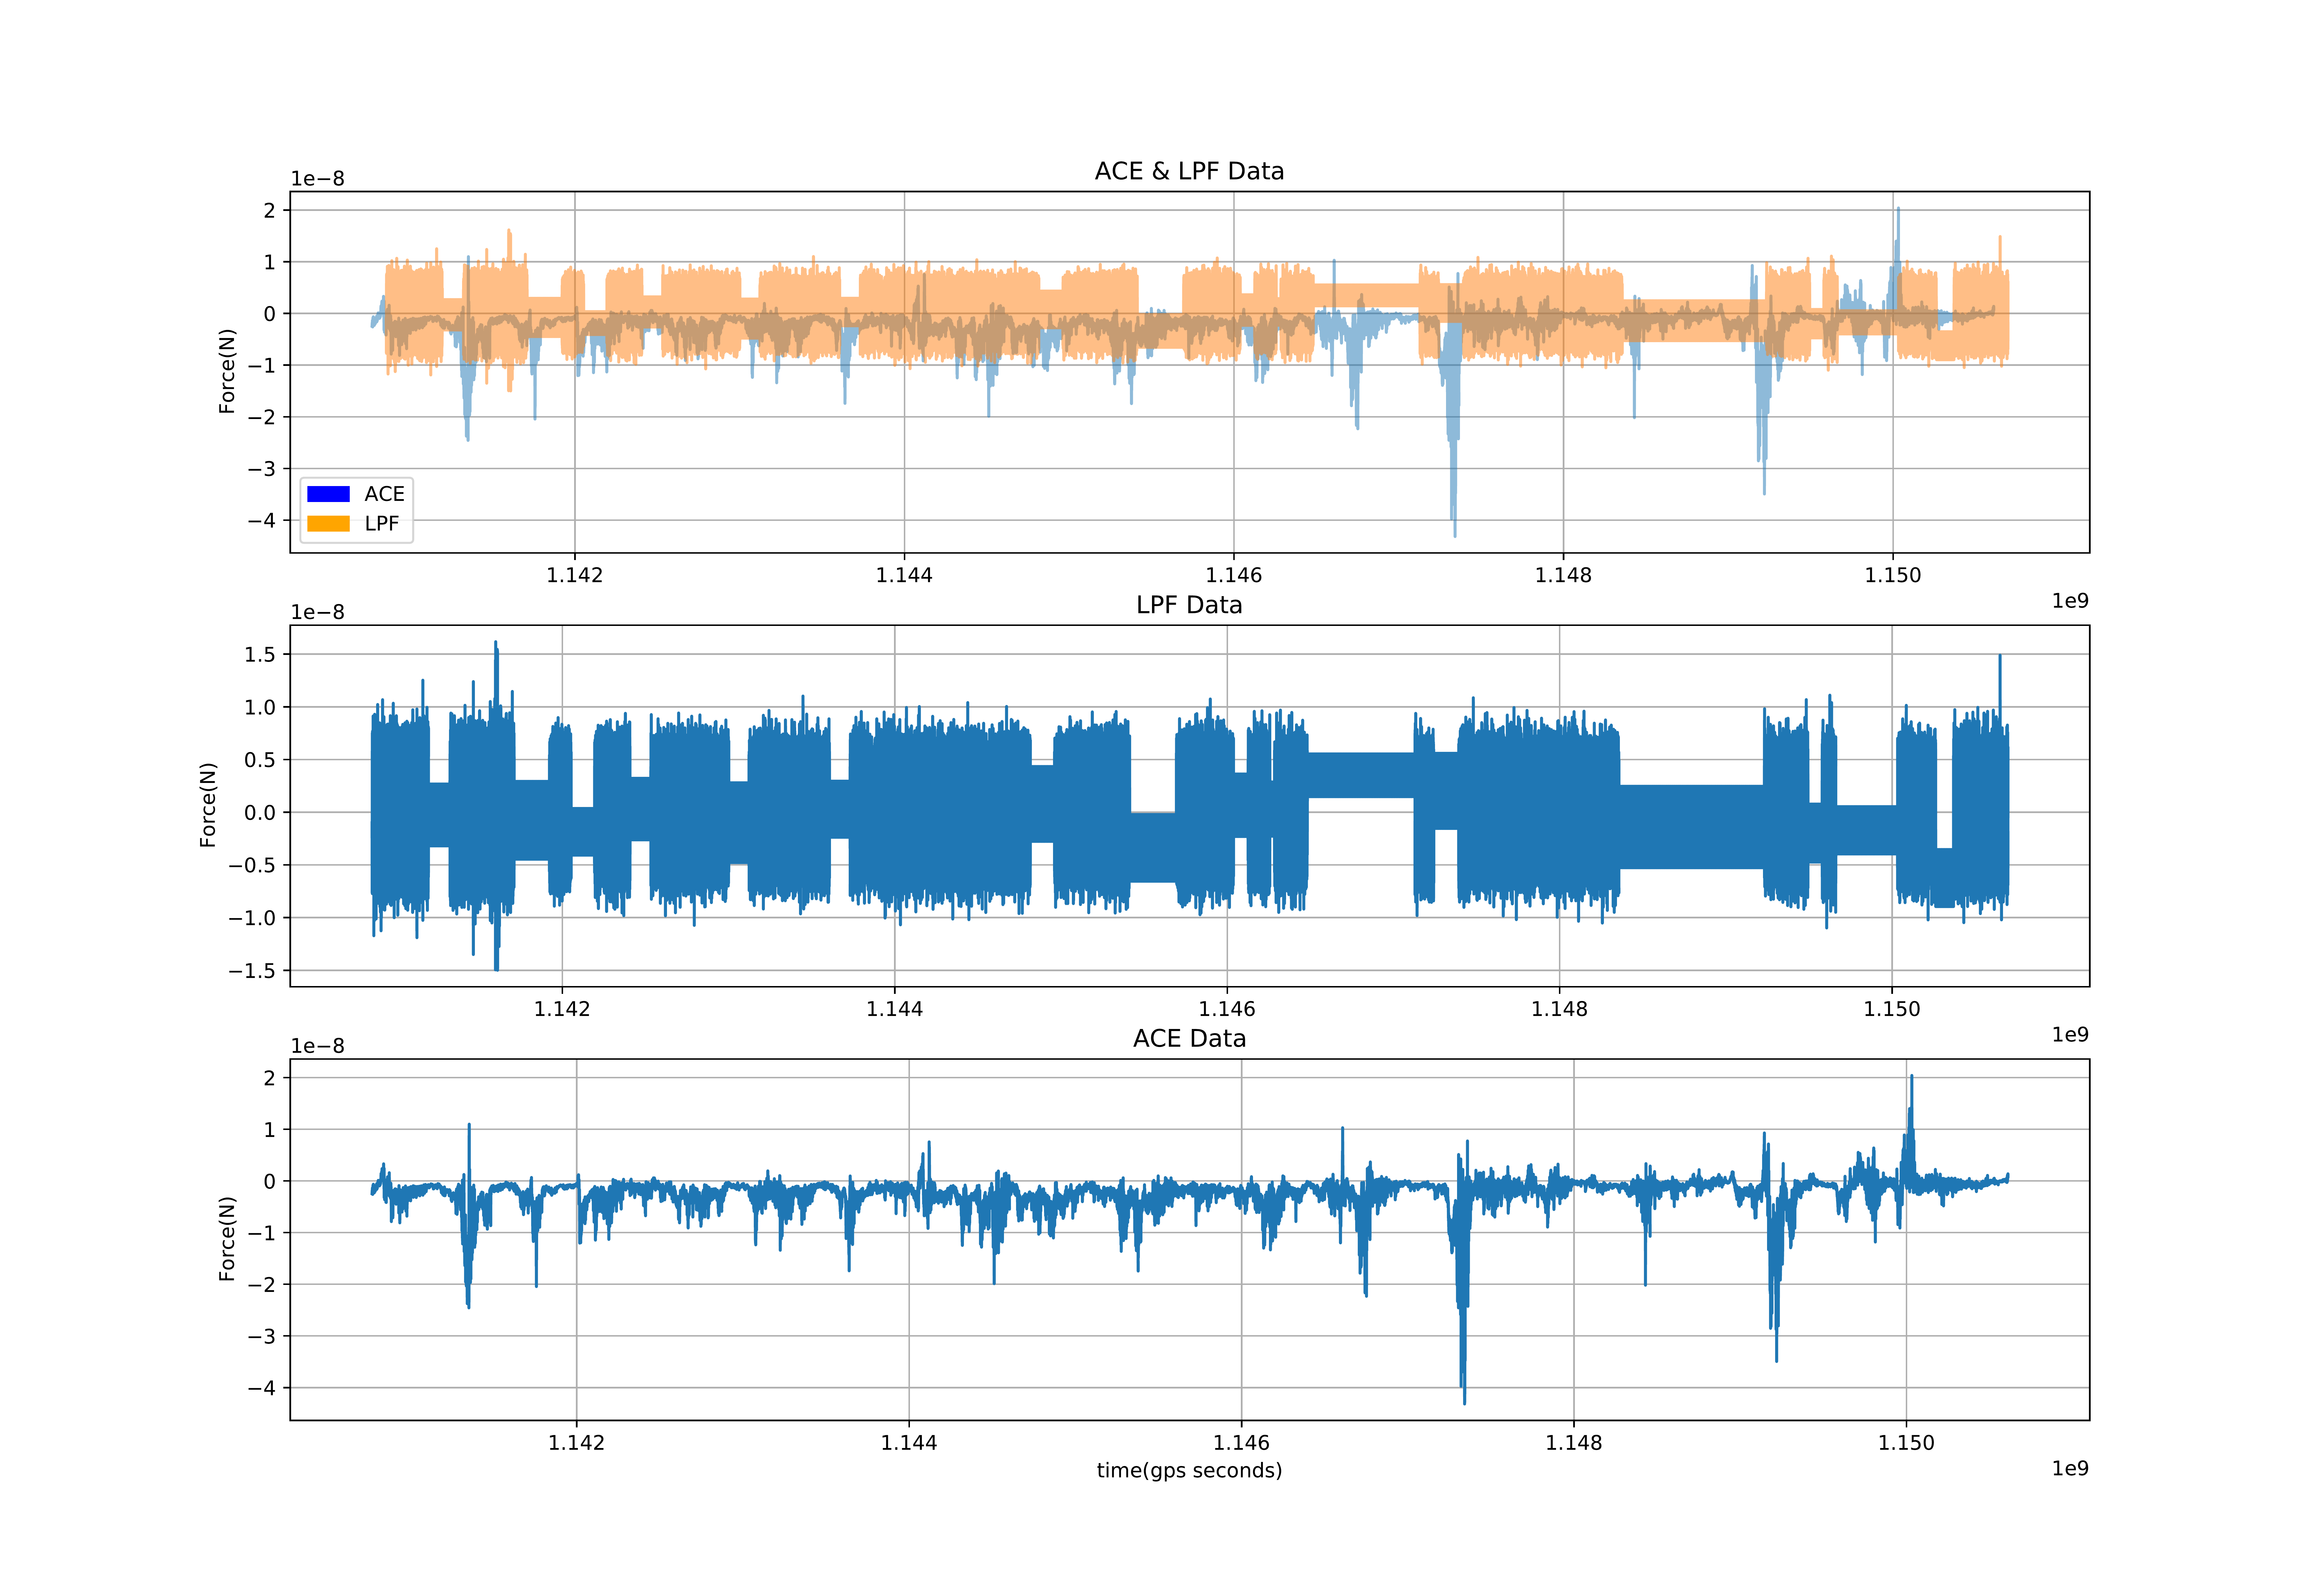
\includegraphics[height=8cm]{TimeDomain_Comparison_ACEvLPF-1.png}
\end{frame}
%------------------------------------------------
\begin{frame}{FFT}
    \centering
    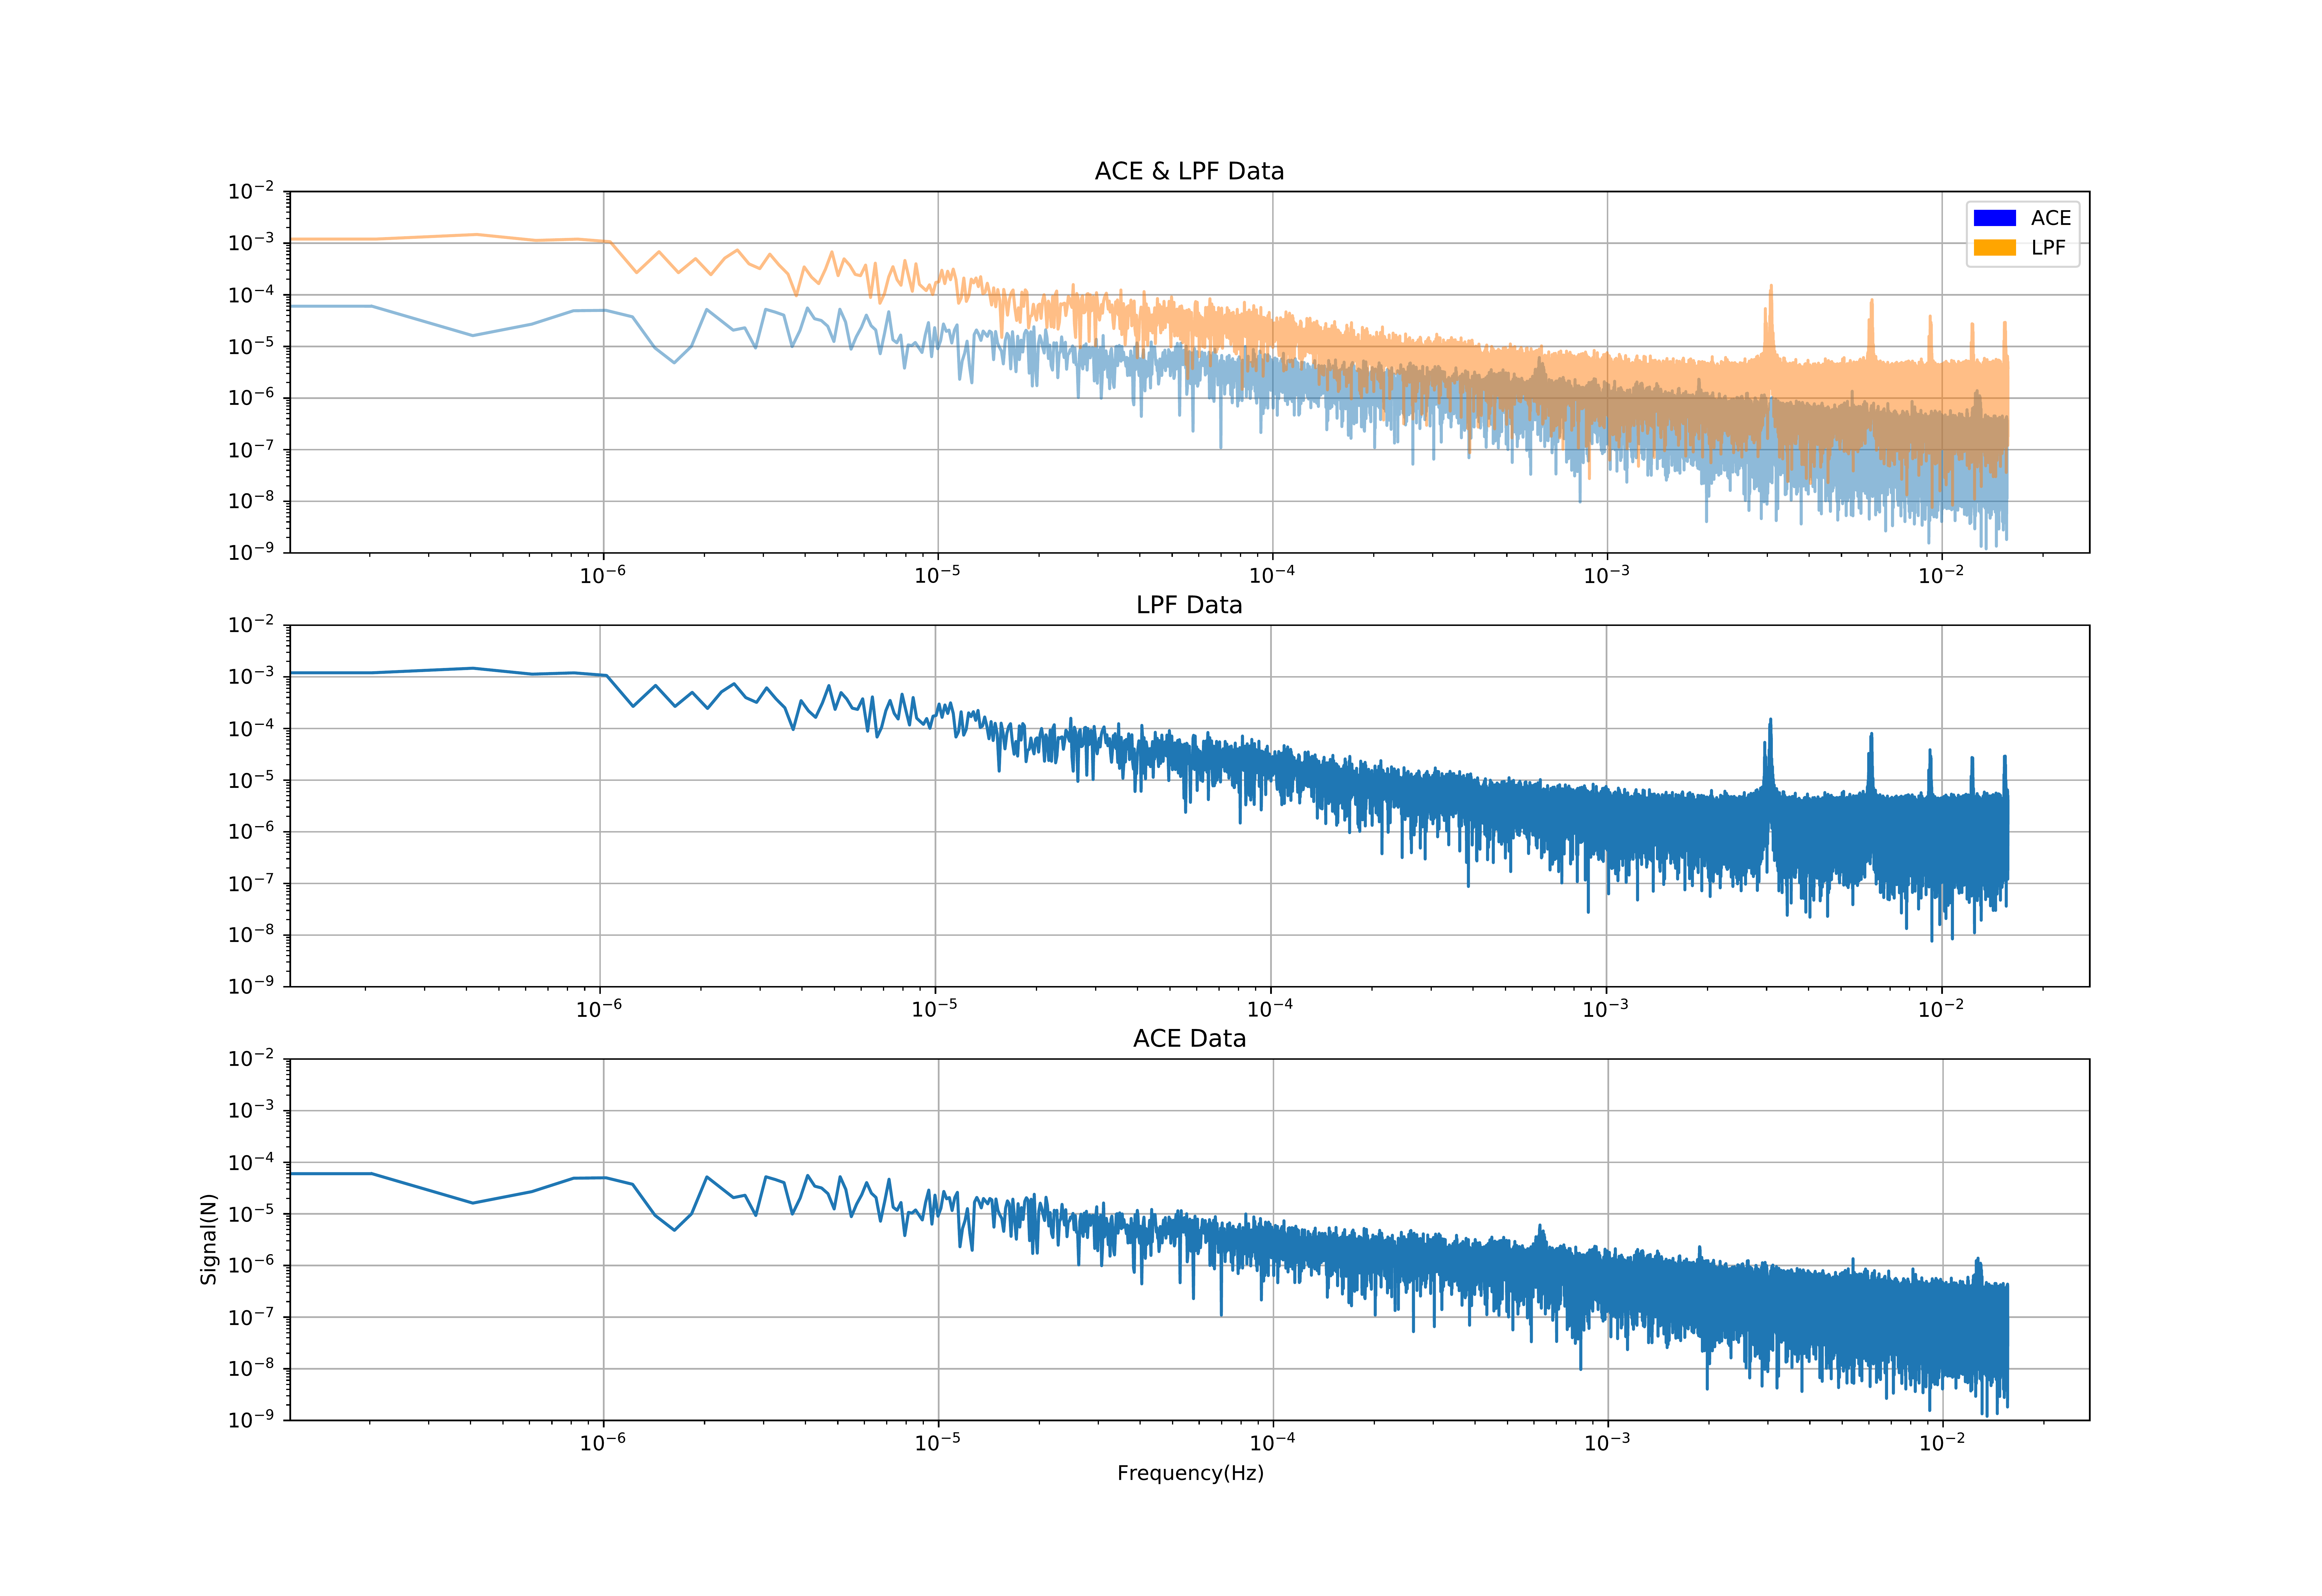
\includegraphics[height=8cm]{ACE_and_LPF_Loglog-1.png}
\end{frame}
%------------------------------------------------
\begin{frame}{Bode Magnitude}
    \centering
    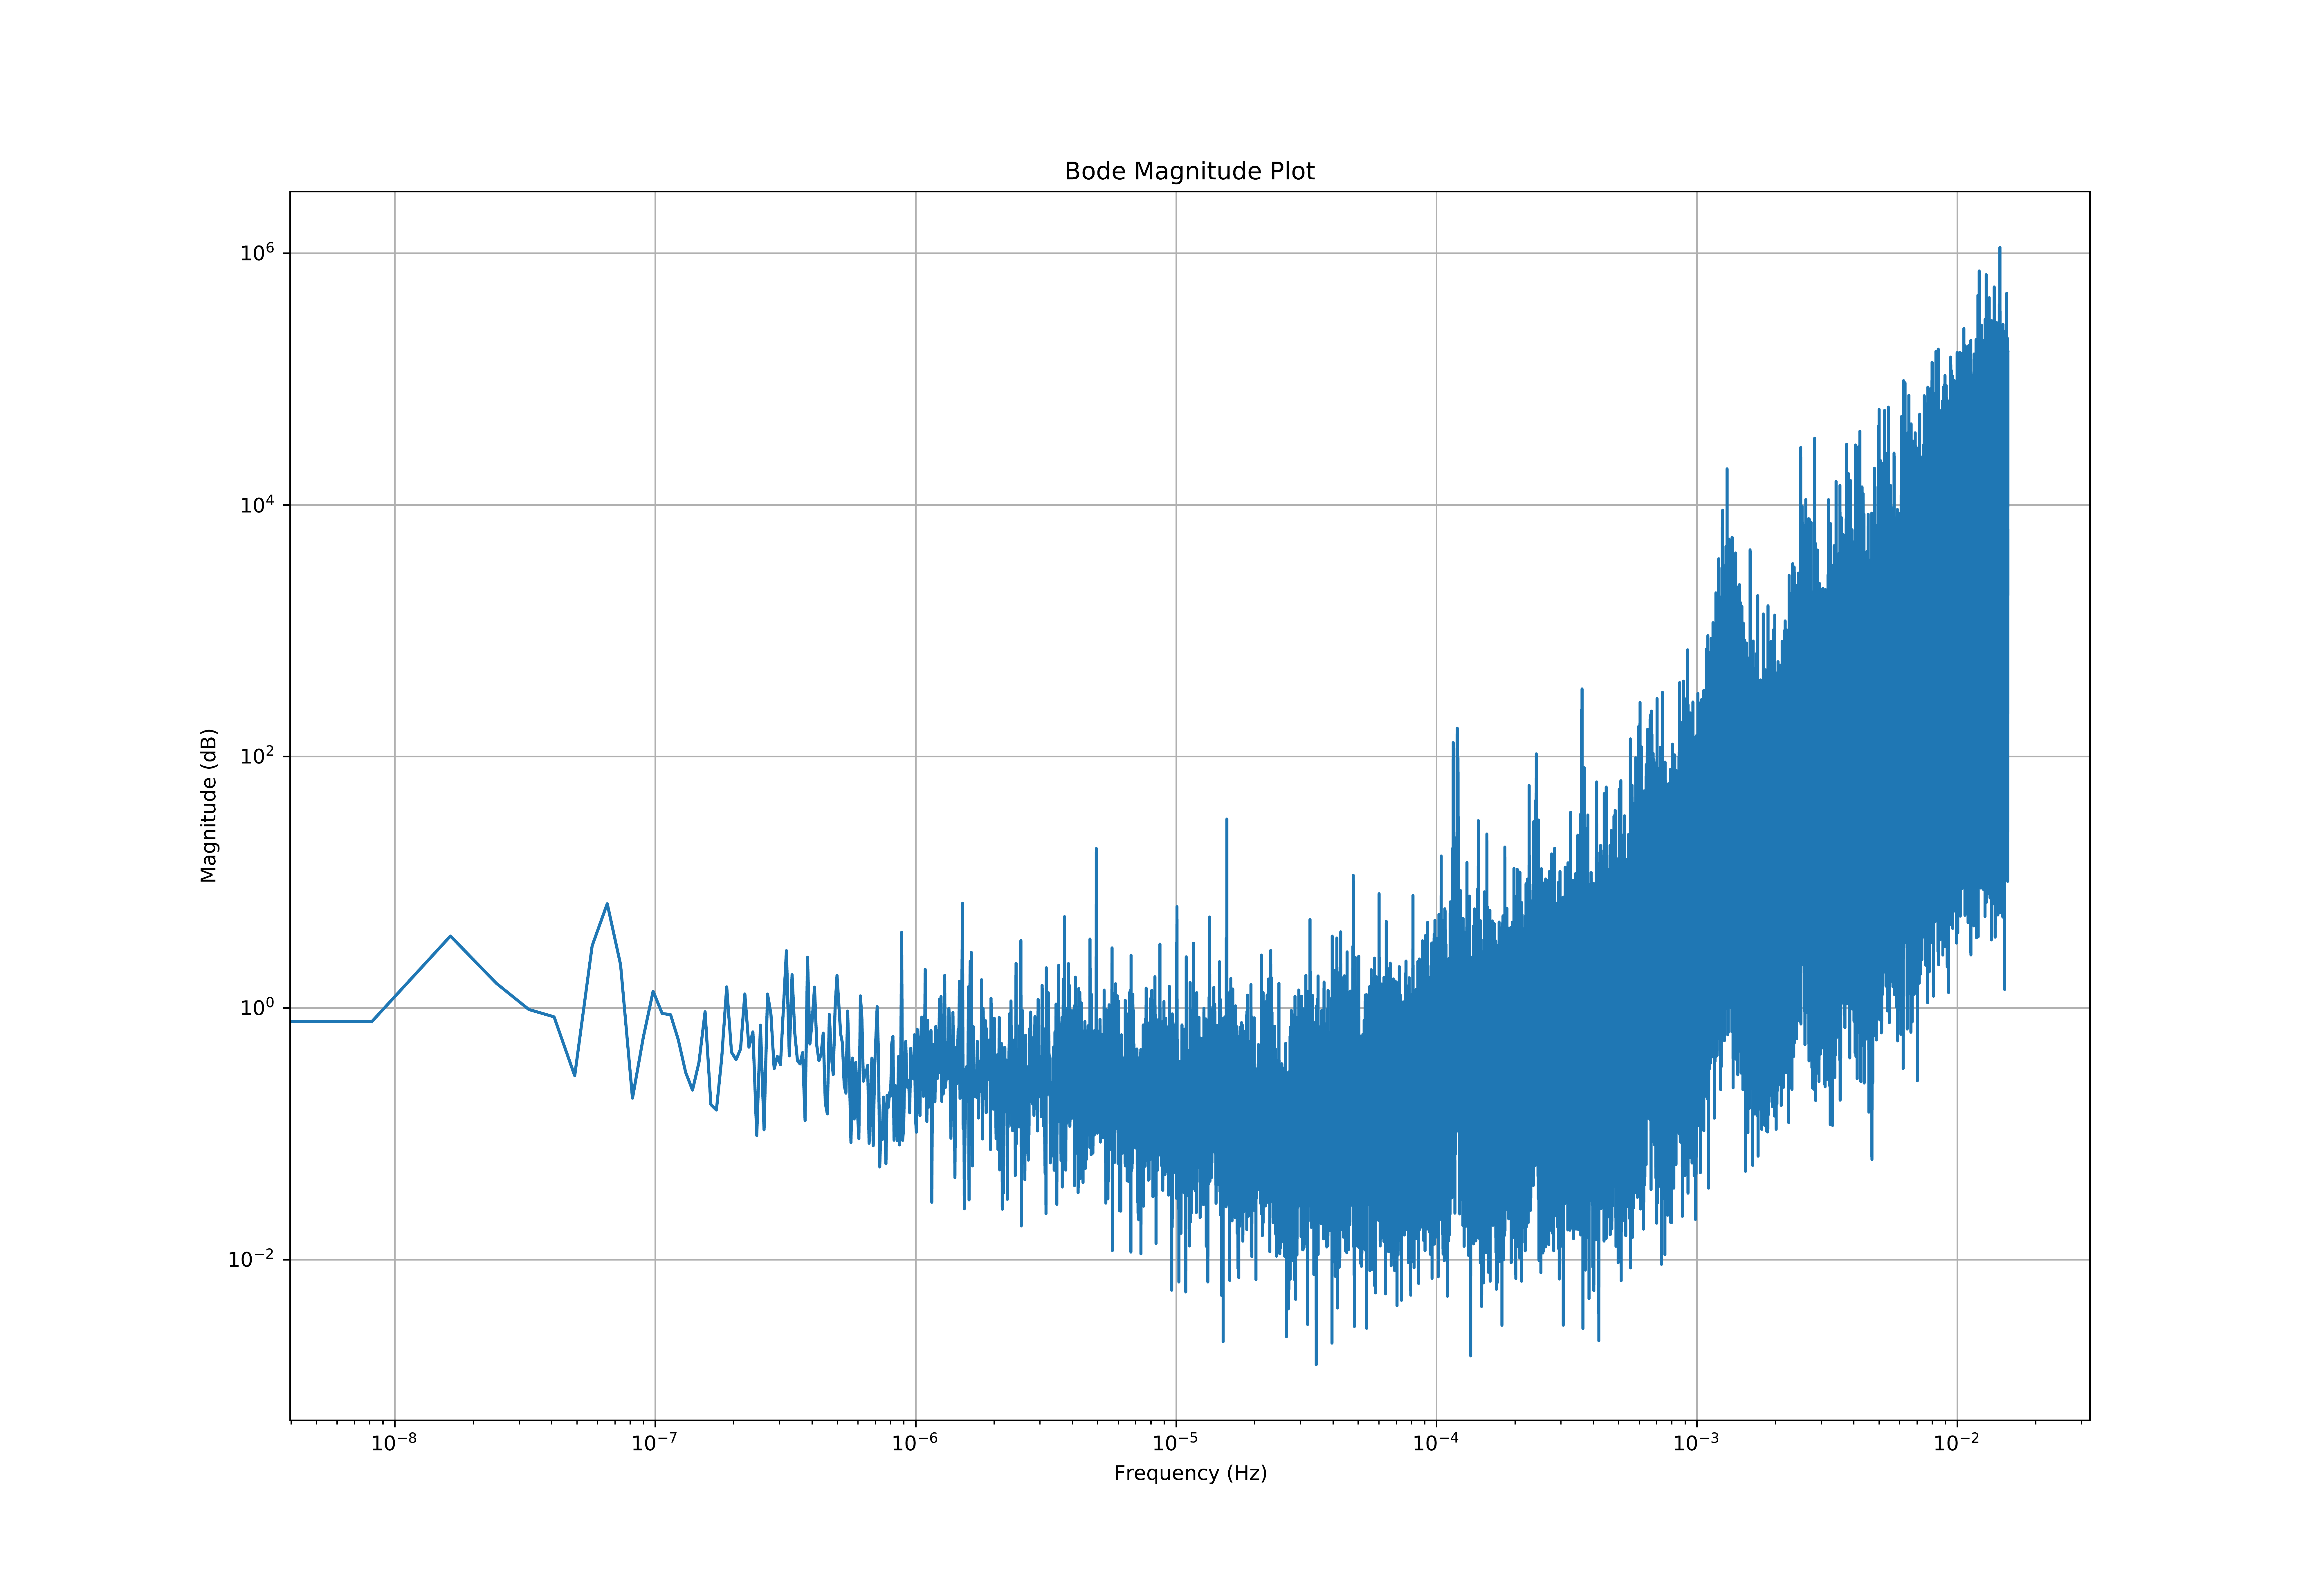
\includegraphics[height=8cm]{Bode_Magnitude_Plot-1.png}
\end{frame}
%------------------------------------------------
\begin{frame}{Bode Phase}
    \centering
    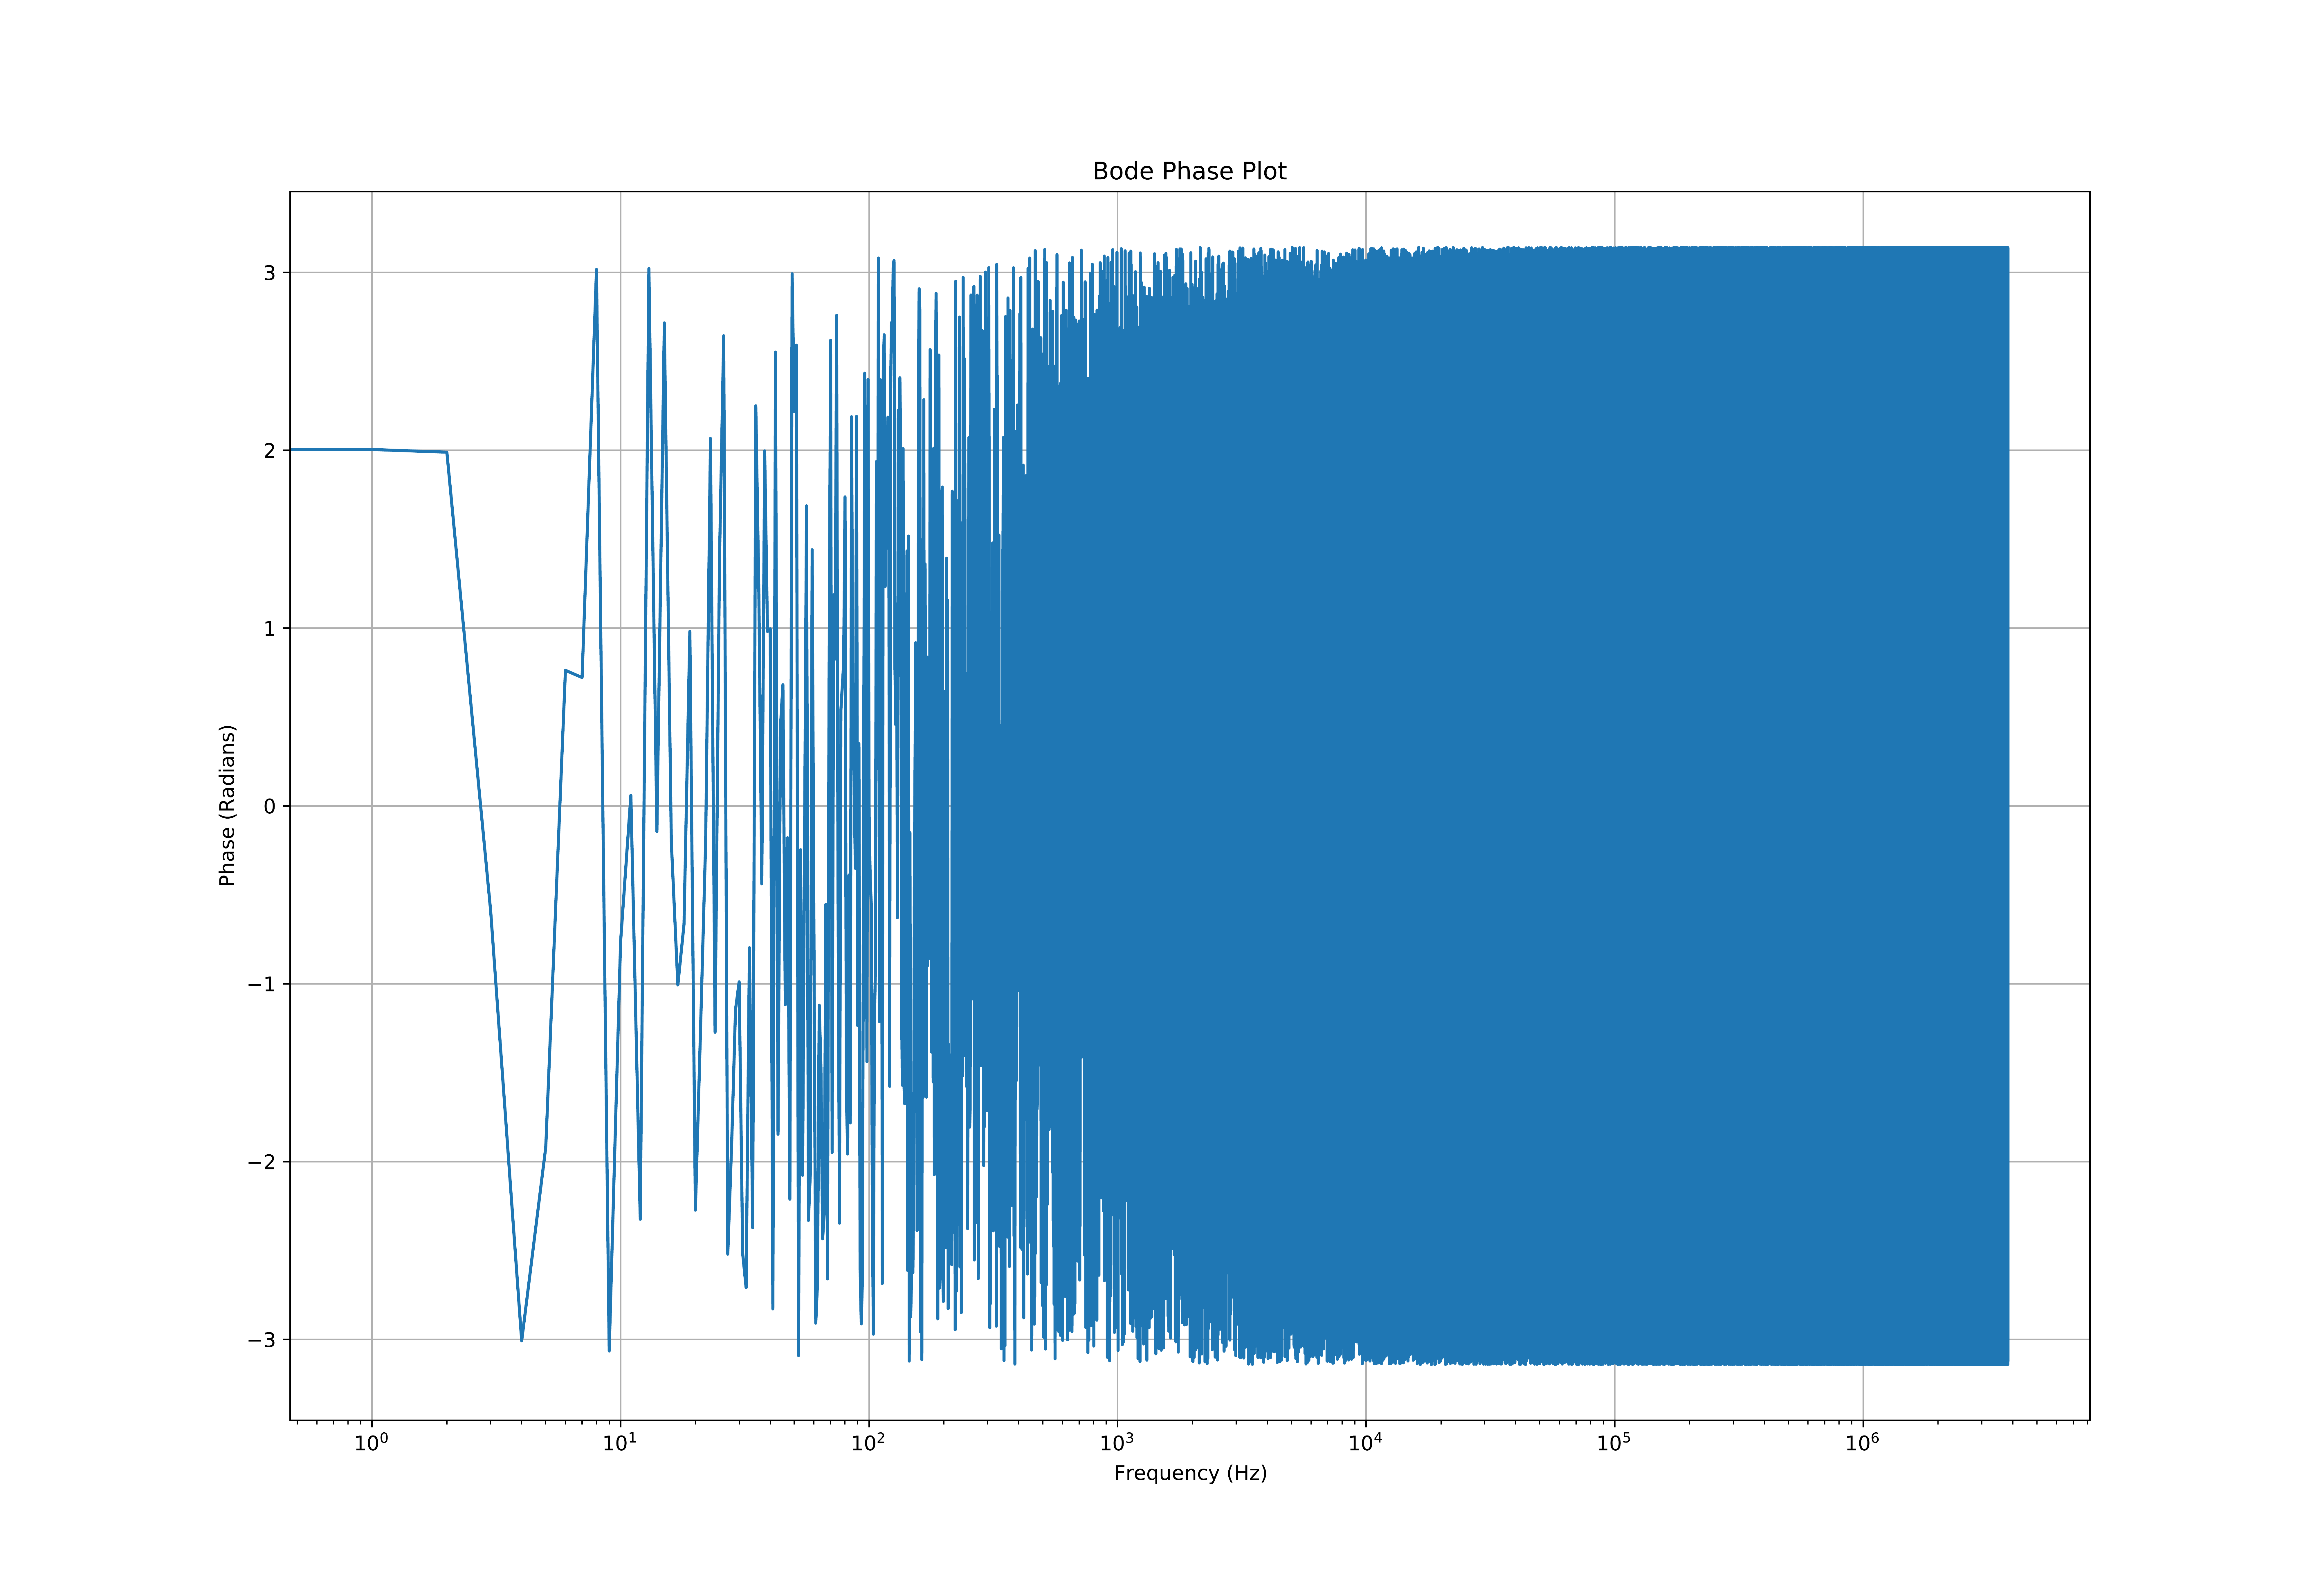
\includegraphics[height=8cm]{Bode_Phase_Plot-1.png}
\end{frame}
%------------------------------------------------
\begin{frame}{Coherece}
    \centering
    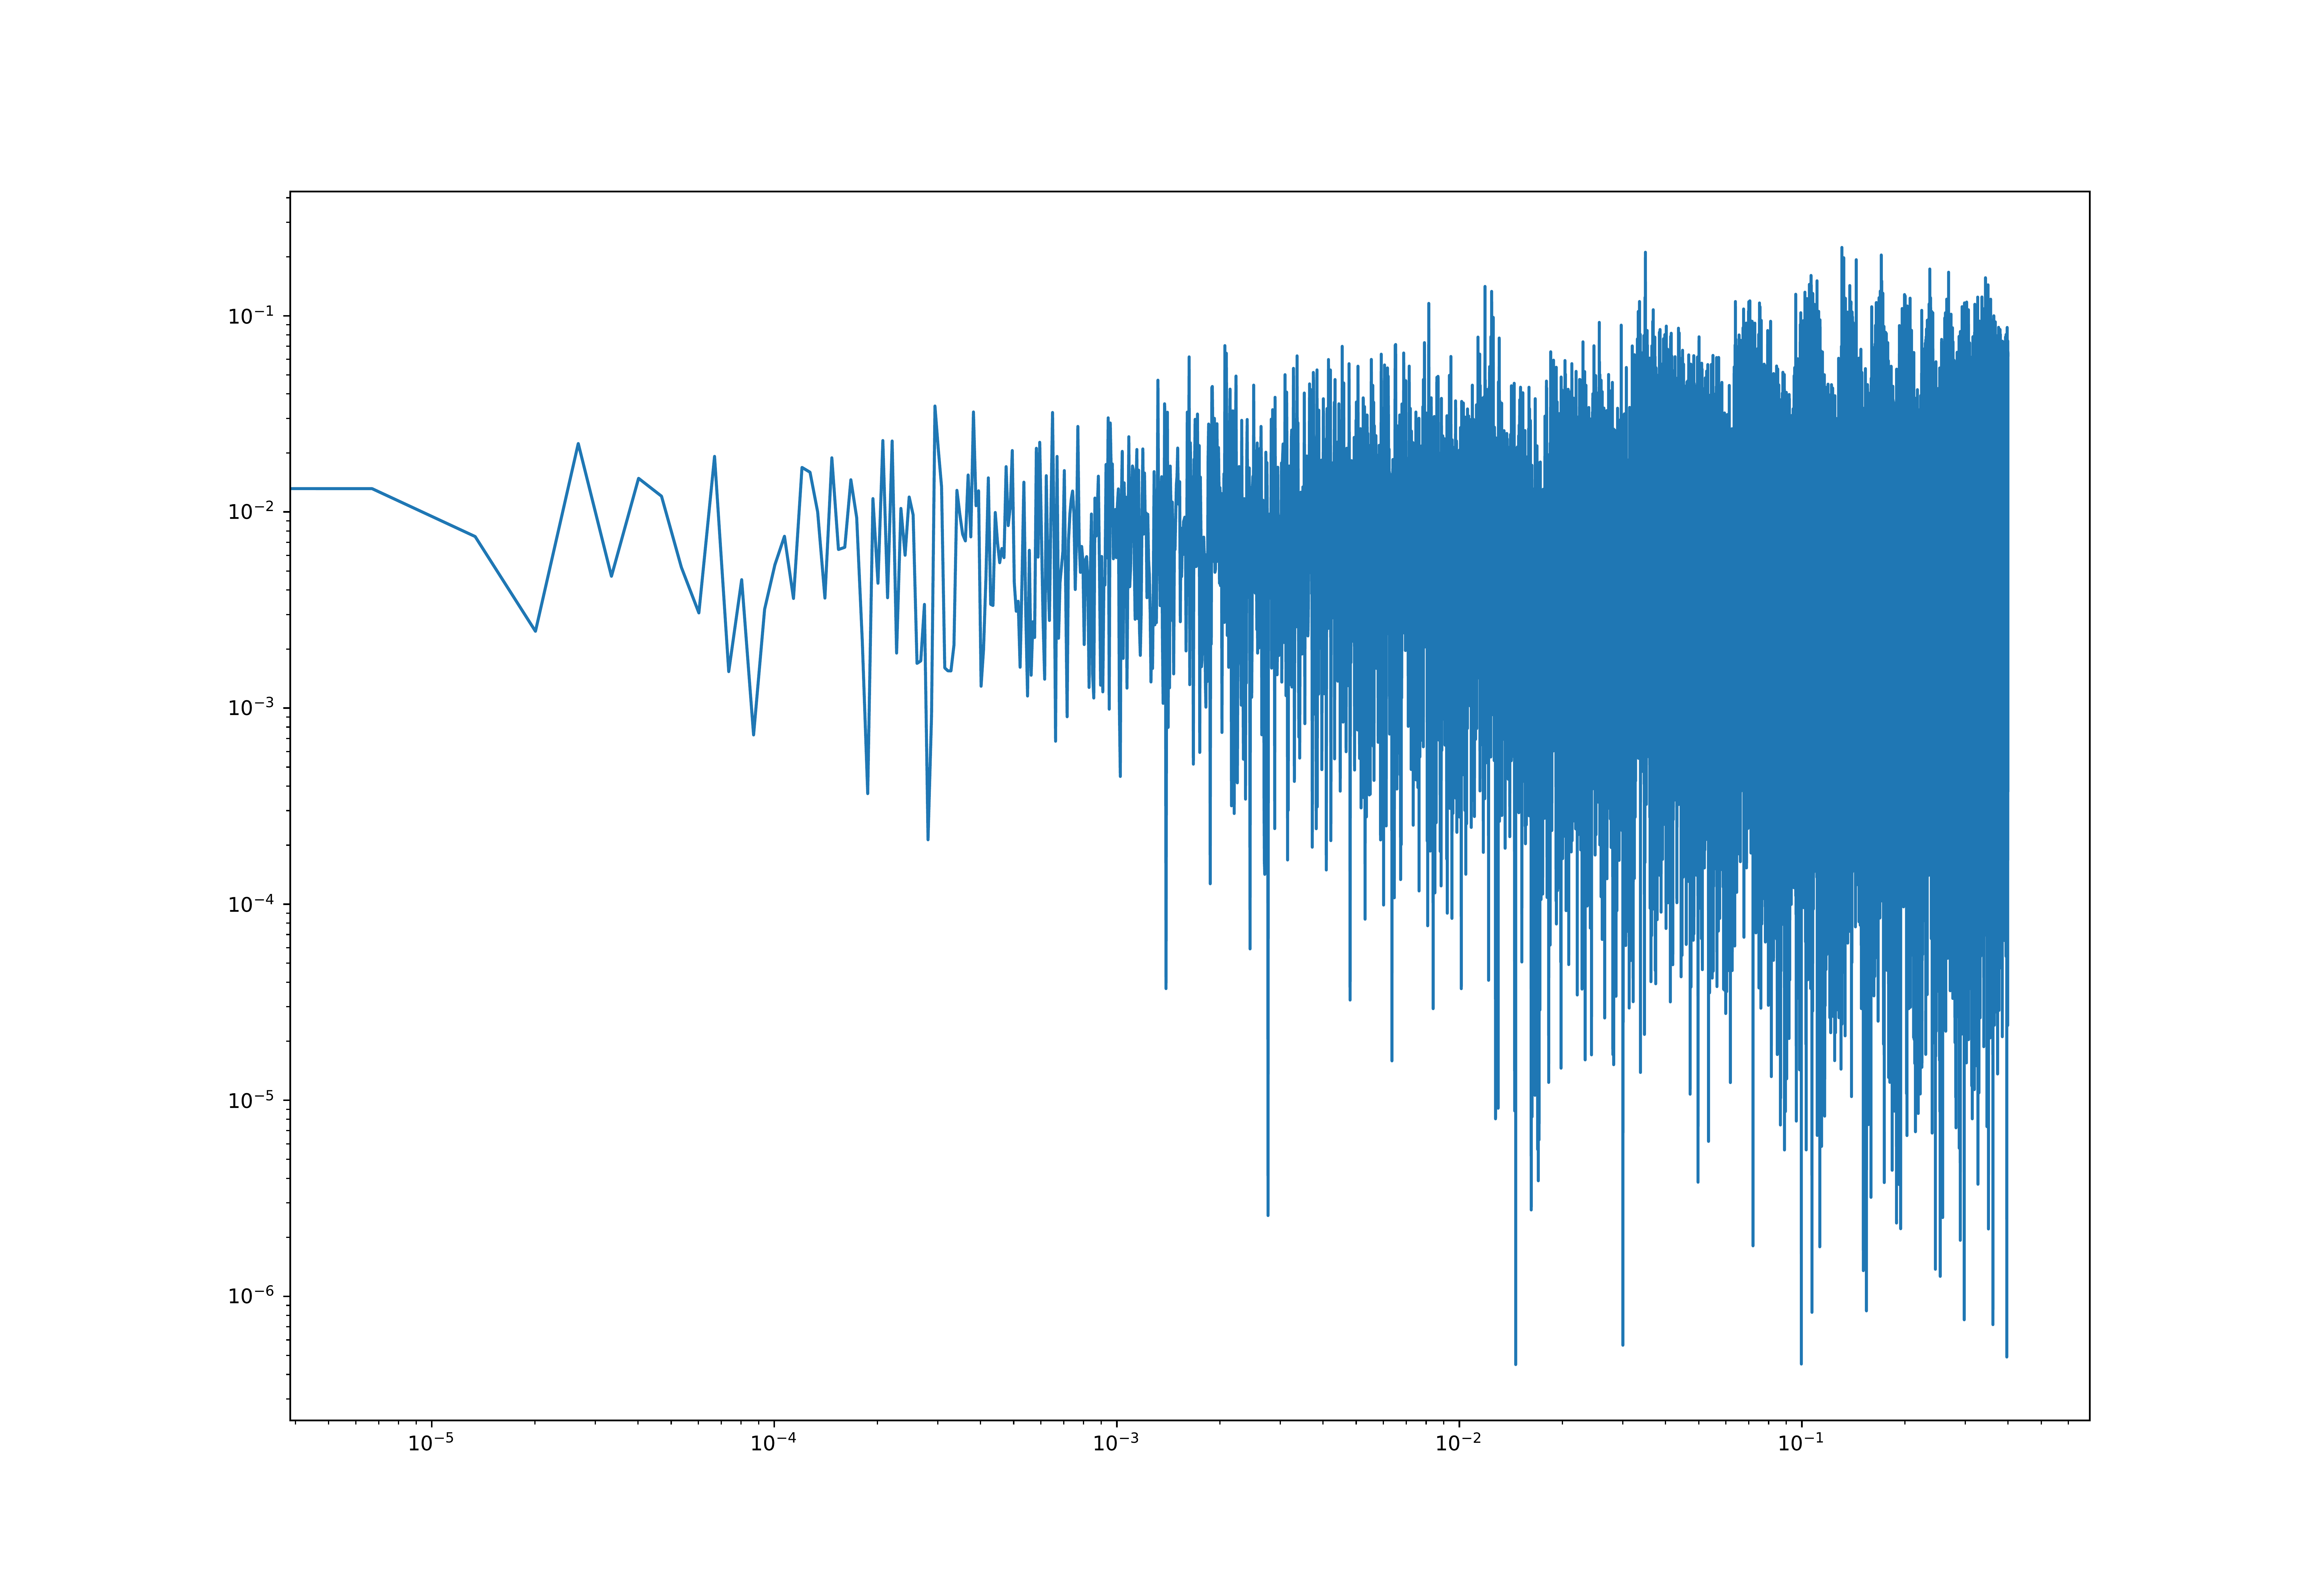
\includegraphics[height=8cm]{ACE_and_LPF_co-1.png}
\end{frame}
%------------------------------------------------
\begin{frame}{Noise Cancellation}
\end{frame}
%------------------------------------------------
\begin{frame}{Conclusion}
\end{frame}
%------------------------------------------------
\begin{frame}{References}
    % Beamer does not support BibTeX so references must be inserted manually as below
    \footnotesize{
        \begin{thebibliography}{99}
            \bibitem[Smith, 2012]{p1} John Smith (2012)
            \newblock Title of the publication
            \newblock \emph{Journal Name} 12(3), 45 -- 678.
        \end{thebibliography}
    }
\end{frame}
%------------------------------------------------

\begin{frame}
    \Huge{\centerline{\textbf{Thank You!!!}}}
\end{frame}
%----------------------------------------------------------------------------------------

\end{document}n
